%Basic Page Formatting%
\documentclass[12pt,twoside]{report}
\usepackage[letterpaper,margin=1in,bindingoffset=0.25in]{geometry}
\usepackage[utf8]{inputenc}
\usepackage[english]{babel}
\usepackage[babel]{csquotes}
\usepackage{titling}
\usepackage[protrusion=true,expansion=true]{microtype}
\usepackage{setspace}
\onehalfspacing
%Chapter Styling%
\usepackage{titlesec}
\titleformat{\chapter}
{\normalfont\Large\bfseries}{\thechapter.}{18pt}{\Large}

%Fancy Page Styling%
\usepackage{fancyhdr}
\pagestyle{fancy}
\fancyhead{}
\fancyhead[RO,LE]{Thesis Title}
\fancyhead[RE,LO]{Chapter \thechapter}
\fancyhead[C]{}
\fancyfoot{}
\fancyfoot[LE,RO]{}
\fancyfoot[C]{\thepage}
\setlength{\headheight}{15pt}

%Reference Management%
\usepackage[
backend=biber,
style=chem-acs,
articletitle
]{biblatex}
\addbibresource{references.bib}

%Image Formatting%
\usepackage{graphicx}%Enchanced graphics support%
\usepackage{float}%Float options$
\graphicspath{{./figures/}}

%Math Formatting%
\usepackage{amsmath}%AMS Math%
\usepackage{amsthm}%Theorem Formatting%
\usepackage{amssymb}%AMS Symbols%
\usepackage{array}%Allows for more complex matrices
\usepackage{siunitx}%Formats SI units%
\usepackage{booktabs}%Typsets tables%
\newcommand{\specialcell}[2][c]{\begin{tabular}[#1]{@{}l@{}}#2\end{tabular}}
\newcommand{\specialcellbold}[2][c]{%
	\bfseries
	\begin{tabular}[#1]{@{}l@{}}#2\end{tabular}%
}

%Lorem Ipsum%
\usepackage{lipsum}

\begin{document}

%Title Page%
\begin{titlepage}
	\begin{center}
		\vspace*{1.5 cm}
		\textbf{\{Working Title\}}


		\vspace{1.5 cm}

		by\\ Benjamin Bui
		\vspace{1.5 cm}

		Professor Peacock-Lopez, Advisor
		\vspace{1.5 cm}

		A thesis submitted in partial fulfillment\\
		of the requirements for the\\
		Degree of Bachelor of Arts with Honors\\
		in Chemistry
		\vspace{1.5 cm}

		Williams College\\
		Williamstown, Massachusetts
		\vspace{1.5 cm}

		\today
	\end{center}
\end{titlepage}


\setcounter{page}{1}
\thispagestyle{plain}
\begin{center}
	\vspace*{\fill}
	\textbf{Acknowledgements}\\
	I would like to express my gratitude to my advisor, Professor Enrique Peacock-L\'opez for supporting me throughout my thesis. It was always helpful to have someone I could bounce ideas off of and to explain to me obtuse math I would find in the literature. You really let me develop and understand the material needed independently but were always there when I needed help. You were the first professor I did research with in the summer of my freshman year and it was a pleasure to work on my thesis with you in my senior year.
	
	I would also like to thank my suite and the people of the Jesup community for providing me with both the emotional and technical support throughout my thesis. You provided the breaks after long hours of work and I look forward to staying close to all of you long after I graduate

	Thank you to the faculty and students Chemistry Department of Williams College. I have worked with, under, or even helped tutored many of you and I hope that you all continue to do fantastic work inside or outside of chemistry. I understand that my thesis appears unorthodox for the department but I thank you all for being understanding and willing to let me work on this. 

	I of course must mention my family who were instrumental in raising me and helping reach the point I am now. Thank you to my mother and father, to my brother and sister: Helen and Bryant, and to the rest of my extended family to whom I love dearly.
	\vspace*{\fill}
\end{center}
\pagebreak
\thispagestyle{plain}
\begin{center}
	\vspace*{\fill}
	\textbf{Abstract}\\
\end{center}
	Dynamical systems are present in a variety of fields including the study of economics, physics and chemistry. The study of stochastic dynamical systems was pioneered by Louis Bachelier\autocite{Bachelier1900} who attempted to model Brownian motion to study financial systems although it was later popularized by Einstein and developed into the theory of statistical mechanics. Econonomic and financial models quickly began adapting these theories into their own models with the field of econophysics being developed in order to accomodate these and related ideas. Many notable processes in chemistry and physics are represented as chaotic dynamical systems; however, chaos is still not a commonplace point of discussion in macroeconomic theory. In this paper, I present two previously created business cycle models, a multiplier-accelerator model with a Robertson lag by T\"onu Puu and an inventory cycle model with a Lundberg lag by Metzler and Wegener, before creating a new model that incorporates these elements from these two models. This model explains the inability for firms to accurately determine future outcomes on the potentially chaotic or quasi-periodic behavior of output levels. I find that even given reasonable parameter choice, it is reasonable for the model to be in a chaotic regime, thus allowing business cycles to be driven endogenously as opposed to through external, stochastic shocks.
	\vspace*{\fill}
\pagebreak
\tableofcontents
\chapter{Introduction}
The study of dynamical systems is traditionally thought to have begun with the publication of "New methods of Celestial Mechanics" by Poincar\'e and expanded with the work of Lyapunov into a theory of the stability of dynamical systems. It was not until the 1960s however that the use of chaos and stability theory exploded across disciplines\autocite{Aubin2002}. 

Dynamics are typically an unnecessary tool when studying the paths of chemical reactions. Their value became apparent however, when Belousov and later Zhabotinsky released published their work on an oscillatory reaction, a reaction that would later come to be known as the BZ reaction\autocite{Winfree1984}. Cycles were also known to exist in the biochemical realm with many famous pathways in organisms such as the Krebs cycle and Calvin cycle; however the BZ reaction was developed to create an inorganic analogue to the Krebs cycle\autocite{Field1986}. The development of this cycle allowed for a relatively easily replicable cyclic reaction with with easily measurable indicators of the progress of the reaction. 

The study of dynamical chemical systems has since expanded to a variety of other mechanisms such as self-replicating molecules\autocite{Beutel2007} in addition to studying fractal patterns and dimensionality involved in electrochemical deposits\autocite{Hudson1994} and flame patterns\autocite{Matalon2009}. Despite the fairly wide range of background information required to set up these different models, the underlying mathematical theory used to study these models is identical which has contributed to the wide range of interdisciplinary work performed by theorists in the field.
\section{Background on Dynamical Systems}
Traditional dynamical systems are modelled in continuous time as a system of ordinary differential equations. These systems typically treat time as the singular independent variable and solve for the evolution of one or more variables in terms of time. A classic continuous time dynamical system is the simple pendulum which allows one to model the movement of a pendulum in space in terms of time. This model uses a variety of simplifying assumptions in order to reduce the problem of the pendulum into a single variable function, holding the length of the pendulum and acceleration due to gravity constant.
\begin{equation}
    \frac{d^2}{dt^2}+\frac{g}{L}\sin\theta=0
\end{equation}
Most  attempts  at  modelling  real-world  systems  however  require  the  use  of  multiple dependent variables in order to effectively model.  However, as the amount of variables increases, the complexity of the model increases.  Modelling and $n$-body system acting on each other gravitationally is of obvious interest in astronomy; however, it was quickly found  that  although  a  1  and  2  body  system  were  relatively  simple  to  solve  for,  the introduction of a third body caused significant complications.  The 3-body system is in fact what Poincar\'e studied in order to develop a theory of chaotic deterministic systems\autocite{Poincare1993}.

That is not to say that these systems cannot arrive at ordered solutions.  Although continuous time systems require a minimum of 3 variables in order for chaos to arise, there are typically windows of order in chaotic regimes that allow for stable, oscillatory behavior. The BZ-reaction is still being actively studied and is known to be actually highly complex but is often reduced into 7 primary sub-reactions\autocite{Field1986}. A great deal of the work involved in studying dynamical systems is actually on finding ways to simplify models in order to arrive at more mathematically tractable systems. The BZ-reaction has been simplified to a 3-variable system that still provides the complex periodicity and chaotic behavior characteristic of the model\autocite{Gyorgyi1992}.

Although many processes in the real-world are more intuitively interpreted as operating as a continuous time  function, there are many  occasions where it is possible and  in fact beneficial to think in a discrete-time sense. The prevalence of this type of system varies depending on the exact field of study; however, it is important to note that when computationally modelling continuous time systems, it is impossible for computers to truly operate with continuous variables and thus even these systems are reduced to technically discrete models.

Population dynamics are frequently analyzed as a discrete time system as opposed to continuous time. It is often of more practical use to interpret $t= 0,1,2,3,...$ as the change in population per year or per season as opposed to determining the change in population over infinitesimally small changes in time. In terms of technique, many of the mathematical principles used in analyzing dynamic systems in continuous time apply to discrete time systems; however, it would be a mistake to assume the two were identical. An important distinction between the two is the nature by which chaos can occur. As described previously, a continuous time system requires 3 or more dependent variables in order for chaos to occur. A discrete time system only requires 1 variable in order to display the same type of chaotic behavior.

The systems discussed throughout this paper will be of the discrete variety due to their nature. Laws pertaining to the physical world are scalable to the infinitesimal degree which allows for their use in continuous models. Economic models do not have a basis in physical laws. It is also important to note that, due to the complexity involved in the human behavior that economic models are trying predict, the exact numerical values of the model are typically of minor concern. The general behavior of the model is significantly more valuable in order to determine the effects of an economic assumption.

The logistic map is regarded as the prototypical chaotic discrete time mapping. The logistic function, which the logistic map is based off of, was developed to study population dynamics but actually garnered widespread use in other disciplines such as the study of autocatalytic reactions, computer science, statistics, and economics\autocite{Kavanagh1934}.
\begin{equation}
    \frac{d}{dx}f(x)=f(x)(1-f(x))
\end{equation}
The logistic function has 2 equilibria or points where the derivative of the function is 0. $f(x) = 0$ is an unstable equilibrium but $f(x)=1$ is a stable equilibrium point which means that other points on the function will tend towards this equilibrium overtime.  This can be realized by solving for the derivative of the function at points when $f(x)\in(0,1)$ which is universally positive and $f(x)\in(1,\infty)$ which is negative. Integrating the differential equation gives the general form equation:
\begin{equation}
    f(x)=\frac{e^x}{e^x+C}
\end{equation}
This function gained prominence due to its rapid, exponential growth when $f(x)$ is low and its slow, linear decaying to non-existent growth as population increases.  Used by notable mathematicians operating in the field of population dynamics such as Verhulst, Pearl, and Lotka, the model continues to be widely used today and is often the basis upon which other modifications are applied\autocite{Zwanzig1973}.

\begin{equation}
    x_{t=1}=\mu x_t(1-x_t)
\end{equation}
The logistic map is a difference equation model popularized by Robert May as a discrete time analogue to the logistic function\autocite{May1976}. When interpreted in the biological context, $x_t$ refers to the ratio of the population at time $t$ compared to the maximal population, thus the mapping is bounded between 0 and 1. Here we see intuitively the major difference between difference equation and differential equation based systems. Differential equations solve for the derivative of a variable with respect to time in terms of the variable, difference equations solve for the actual state of the variable in the successive state provided we know the state of the variable in the previous time period. Much like how differential equations can be of higher order with the introduction higher order derivatives, a difference equation can also be of higher order by including more time periods in the function for the state of the variable which is valuable in a variety of the models discussed later.

Much like how the equilibrium points were solved for in the differential equation, difference equations also have equilibrium points where $x_{t+1}=x_t$. Interestingly, unlike the logistic function, there does not exist a fixed point at $x_t=1$ as this would result in $x_{t+1}=0$. Solving for the fixed points, we have:
\begin{equation}
    x_{t+1}=x_t=0,\frac{\mu-1}{\mu}
\end{equation}

The stability of a fixed point is again dependent on the derivative of the function; however, there are differences in the details of our analysis. Treating $f(x)=x_{t+1}$, we see the derivative of the logistic map is:
\begin{equation}
    f^\prime(x)=\mu(1-2x)
\end{equation}
For reasons that will become clear later, the stability of a point on the map requires that $|f^\prime(x)|<1$. Solving for when this is true for our two fixed points, we see that $\mu<1$ provides stability for the origin fixed point and $1<\mu<3$ gives stability for the non-zero fixed point. Thus, provided the parameter $\mu$ satisfies either of the conditions set previously, it will converge to one of the fixed points in a relatively small, finite amount of iterations. 

\begin{figure}
    \centering
    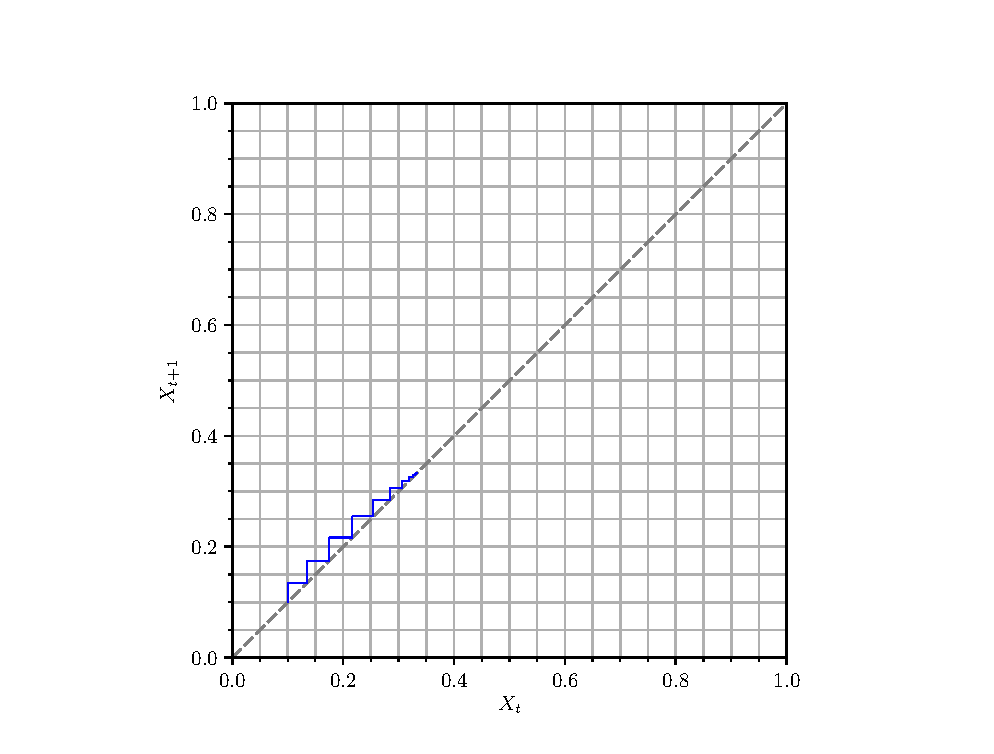
\includegraphics[height=0.4\textheight]{./logistic/fixed_cob.eps}
    \caption{Cobweb plot of the logistic map setting $\mu=1.5$ and $x_0=0.1$. The trajectory asymptotically approaches the equilibrium point of $\frac{1}{3}$.}
    \label{log_fixed_cob}
\end{figure}

This behavior can be visualized using a cobweb diagram. This diagram consists of 3 primary elements: a plot of the mapping, a \SI{45}{\degree} line, and a plot of the variable's trajectory. An example of a cobweb diagram can be seen in Figure \ref{log_fixed_cob}. This diagram shows the trajectory of $x$ starting at a value of 0.1 when there is a stable, non-trivial fixed point.

The \SI{45}{\degree} line is defined as the line where $x_t=x_{t+1}$ which is useful for determining the result of successive iterations. Beginning from the point $x_0$, we can then determine what point $x_1$ wll be via the mapping. We can then look horizontally to the \SI{45}{\degree} line until we intersect with it. The $x$-coordinate of this intersection point is equivalent to the result of the mapping of the previous iteration, thus using this new point will allow us to determine the result of the next iteration of the function. This process can be repeated ad infinitum; however, the result will soon prove uninteresting for stable points and orbits as the trajectory will converge and repeat its behavior.

The reason the logistic map is so frequently studied is because of its ability to exhibit complex behavior beyond a stable equilibrium solution. Once $\mu>3$, the mapping enters a cyclic region. Much like how fixed points could be solved for by identifying where $x_{t}=x_{t+1}$, stable oscillatory points can be found by solving for the equilibrium points of higher iterations of the function. A 2-cycle will be such that $x_{t}=x_{t+2}\neq x_{t+1}$ for example and the stability of a such a cycle can be found using the same methodology as described previously. 
\begin{figure}
    \centering
    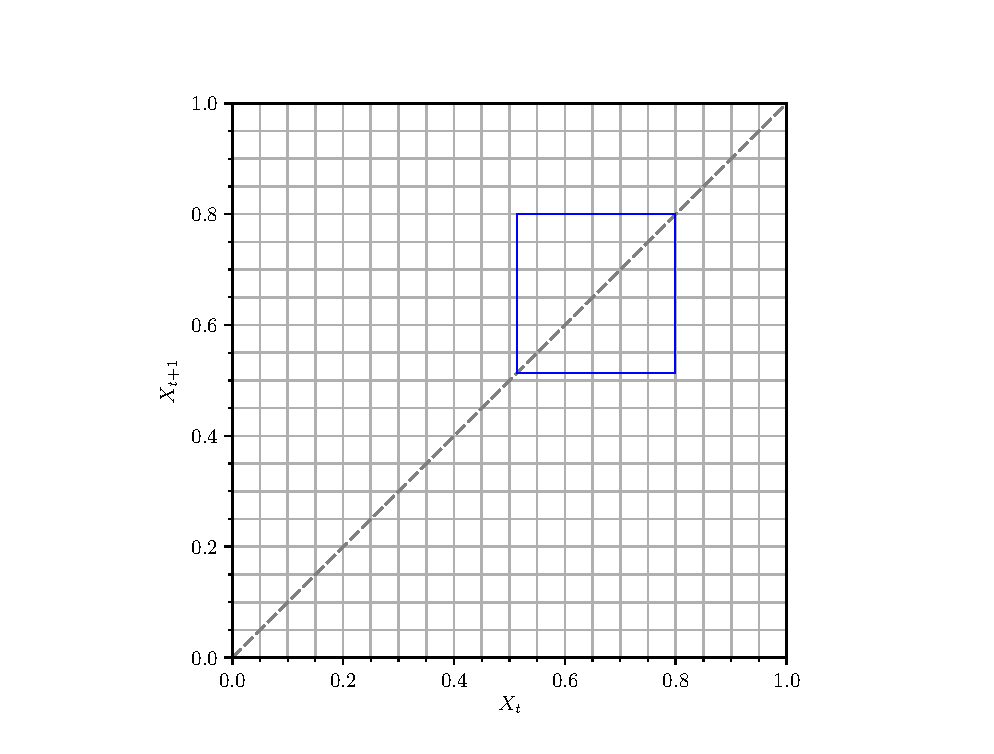
\includegraphics[height=0.4\textheight]{./logistic/2-cyclic_cob.eps}
    \caption{2-period cycle of the logistic map showing only the cyclic behavior.}
    \label{log_cyclic_cob}
\end{figure}
The logistic map also provides a mechanism to more quantitatively describe what it means for a system to be chaotic. The Lyapunov exponent, named after one of major driving forces in the development of stability analysis, is used to measure the effect of small perturbations in initial conditions on the trajectory of the variable\autocite{Puu2003}. Conceptually, the logistic map and the systems discussed in this paper are deterministic. However, chaotic systems have highly divergent trajectories with even small changes in their initial conditions; thus knowing approximately what the initial conditions are does not provide approximate information on the trajectory of the variable. 
\begin{figure}
    \centering
    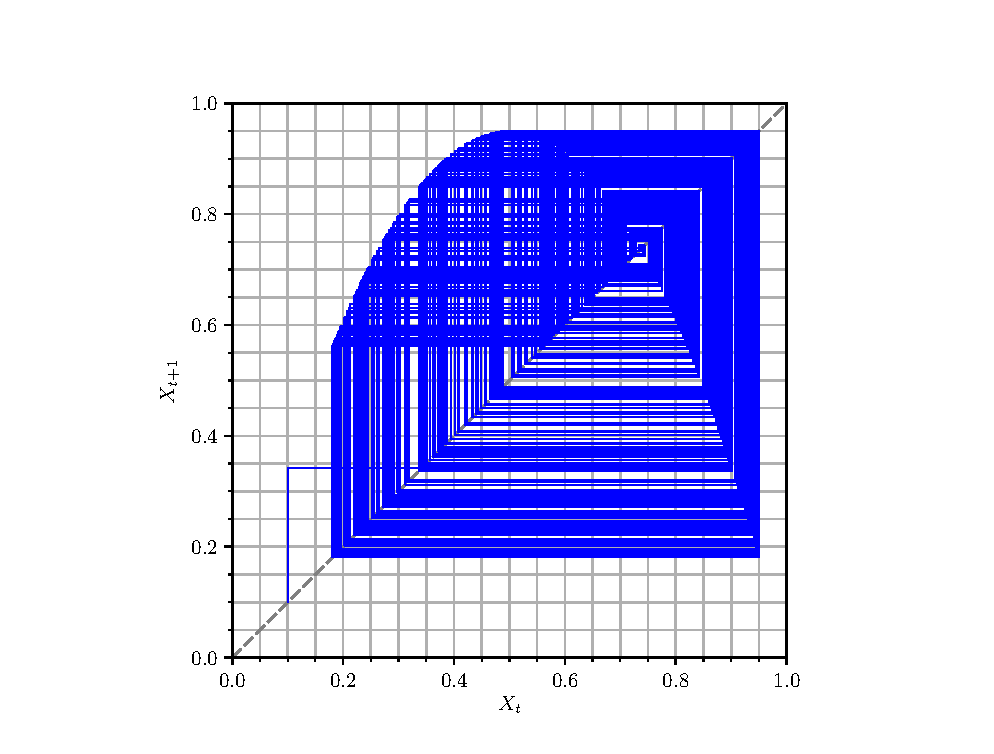
\includegraphics[height=0.4\textheight]{./logistic/chaos_cob.eps}
    \caption{Chaotic behavior in the logistic map.}
    \label{log_chaos_cob}
\end{figure}

In order to quantify this, we begin by taking the absolute value of the derivative of the function as this allows us to effectively magnify the effect of an infinitesimal change in the initial conditions. We then take the natural logarithm of this derivative in order to measure the exponential rate of separation of trajectories. Finally, we take the average separation over an arbitrarily high number of iterations $n$ as exponential separation is not necessitated over all phase space. This gives us a the equation:
\begin{equation}
    \lambda_n(x_0)=\frac{1}{n}\sum^{t=n}_{t=1}\ln\lvert f^\prime(x_{t-1})\rvert
\end{equation}
where $\lambda_n(x_0)$ is the lyapunov exponent for a given initial point when allowed to run for $n$ iterations. The true value of the lyapunov exponent is the limit of the infinite series as $n\rightarrow\infty$ divided by $n$; however, the complexity of these maps often makes it practically impossible to analytically solve for the limit. By choosing arbitrarily high values of $n$ though, it is possible to achieve better approximations at the expense of computational time. It is also important to note that, although the lyapunov exponent is a function of the initial condition, as long as the initial state is not in some stable fixed point or cycle, the trajectories will follow that of the chaotic attractor, thus the value of the lyapunov exponent should be mostly consistent regardless of the choice of initial conditions.
\begin{figure}
    \centering
    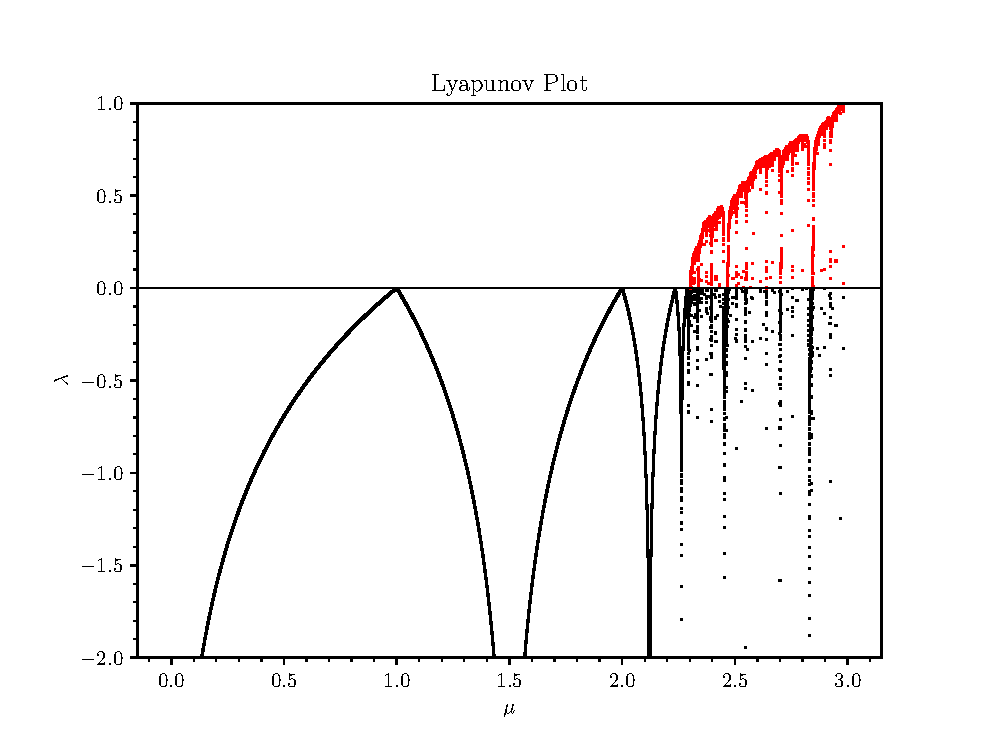
\includegraphics[height=0.4\textheight]{./logistic/lyapunov.eps}
    \caption{Lyapunov exponent plotted against $\mu$ for the logistic map. Initial value of 0.1 is used. Red denotes regions where $\lambda\geq0$, black denotes regions where $\lambda<0$.}
    \label{log_lyapunov}
\end{figure}

Another way visually see the behavior is with a bifurcation diagram. This diagram shows the long run behavior of the variable for a given variable. Figure \ref{log_bifurcation} qualitatively shows the behavior described previously. For parameter values between 0 and 1, we see the origin fixed point is stable. For parameter values between 1 and 3, their is still a single fixed point that is monotonically increasing; however, we can also clearly see the beginning of the 2-period cycle once the parameter exceeds 3. It is difficult however, to determine when predictable higher-order cyclic behavior ends and chaotic behavior begins via qualitative observation of the bifurcation diagram. The benefit of the bifurcation diagram is that it allows us to see both where the bifurcation points are and what behavior the bifurcation points signify. Bifurcation points are 
where where infinitesimally small quantitative changes in the parameter induce significant qualitative or topological change in the behavior of the mapping such as the transition from a stable fixed point to a 2-period cycle. 
\begin{figure}
    \centering
    \includegraphics[height=0.4\textheight]{./logistic/bifurcation.eps}
    \caption{Bifurcation diagram plotting $x$ against $\mu$ for the logistic map.}
    \label{log_bifurcation}
\end{figure}

Research on the logistic map and other iterated maps has shown the existence of what is called Feigenbaum's constant. This constant can be found by observing the behavior of the periodic cycles of the map. The interval of stability decreases and the ratio of subsequence intervals actually approaches a limit $\delta\approx4.6692$\autocite{Puu2003}. All other topologically similar maps with a single local maximum share this Feigenbaum constant. Once the mapping exceeds this constant, chaos occurs which allows for another method to determine precisely where chaotic behavior occurs. 

It is also beneficial to point out that another mechanism exists for cyclic behavior to exist. The previously described method involved taking a mapping and solving for the stability of its double iteration. This allows for $2n$-period stability cycles to exists. However, there does exist odd-ordered cycles such as the $3$ cycle; however, it occurs as a window of order in the region of chaos. These windows can be seen in Figure \ref{log_lyapunov} where the Lyapunov exponent dips into the negative region past the chaotic bifurcation point. These bifurcation points are known as tangent bifurcations.
\begin{figure}
    \centering
    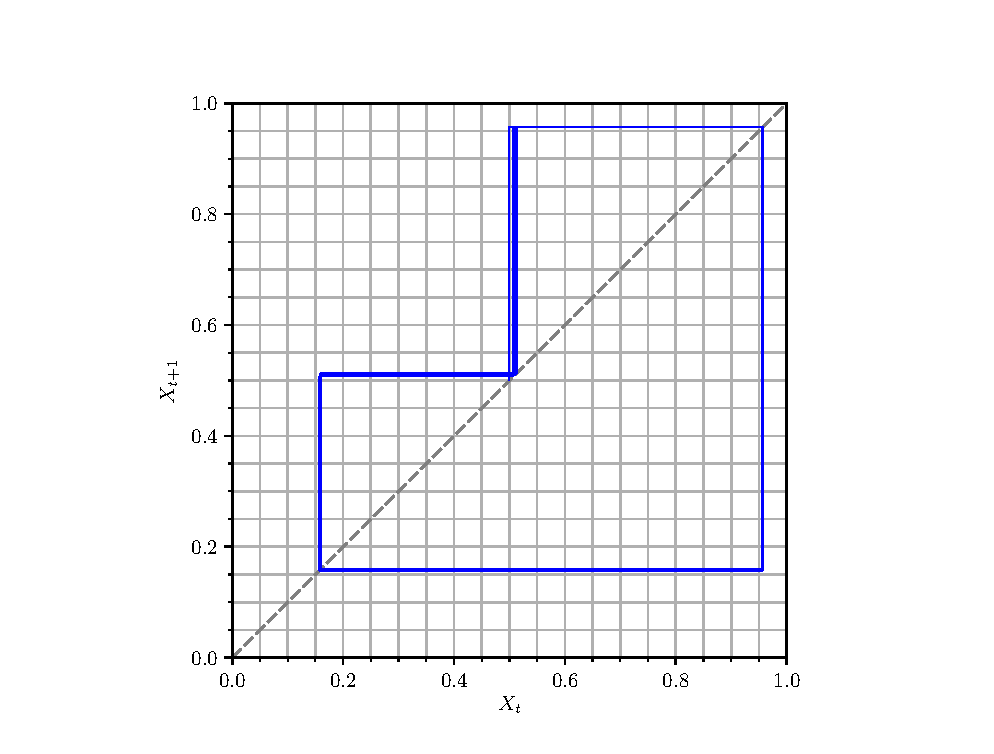
\includegraphics[height=0.4\textheight]{./logistic/3-cyclic_cob.eps}
    \caption{3-period cycle of the logistic map showing only the cyclic behavior.}
    \label{log_3-cyclic_cob}
\end{figure}
This also allows us to use Sharkovsky's Theorem, which states that any continuous mapping with a 3-period cycle must also have every $n$-period cycle for every $n\in\mathbb{Z}$.\autocite{Puu2003} A variety of other mathematical techniques exist to study the dynamics of difference equation mappings but these will be covered more specifically when used for the specific case. 




\chapter{The Multiplier-Accelerator Model}
\section{Background}
John Maynard Keynes work revolutionized economic thought; however, he never formalized any of his theories into a mathematical theory. This was performed in a process known as the neoclassical synthesis which was so called for its attempt to bridge classical models with these Keynesian principles. Paul Samuelson and Sir John Hicks were deeply influential in summarizing Keynesian macroeconomics into mathematically tractable models and their work was incorporated into a discrete-time business cycle model by T\"{o}nuu Puu\autocite{Puu2003}. Key to the theory of the model are the concept of a multiplier and accelerator.

Keynes espoused the idea that increasing spending in the economy by some amount $x$ actually increased the national output by an amount $>x$. In essence, the effect of increased spending was actually multiplied by a positive amount. Although this was originally studied in order to determine the effects of changes in government spending in order to inform fiscal policy\autocite{Samuelson1939}, the principle of the mechanism impacts all forms of expenditure in the economy. 

Integral to the rise of cyclic dynamics in the model is the presence of the Keynesian accelerator which actually makes use of the multiplier effect. The effect can be best explained via example: suppose there is a general increase in national output level. This increases business profits and expectations, thus inducing them to increase investments. This further increases output via the multiplier effect, causing an accelerating level of growth. The same occurs if the economy depresses as businesses will decrease investment due to falling prospects\autocite{Jorgenson1963}

The combination of these two mechanisms, typically referred to as the multiplier-accelerator effect, are sufficient in creating a stable cyclic or even chaotic economy as opposed to a static steady-state model. This type of model allows for cyclic behavior to occur endogenously, that is to say the model allows for persistent behavior outside of the steady state. This idea runs contrary to the idea that economic booms and recessions are reactions to exogenous shocks which is common in the new classical models. Also known as freshwater economics, these models assume that agents are perfectly rational and are capable of learning from past experiences. This viewpoint came into prominence in the late 1970s with a model by Lucas and Sargent\autocite{Lucas1979} which sought to move past these seemingly outdated Keynesian principles. In the modern day however, Keynesianism has regained popularity with a new neoclassical synthesis that resulted in a new school of thought, New Keynesianism, that seeks to provide stronger micro-foundations to macroeconomic models than was previously encountered in neo-Keynesianism. 
\section{Model Set-up}
The model presented here is identical to that presented by T\"onu Puu\autocite{Puu2003}. The first factor of the economy to consider is that of investment. In order for investment to operate under Keynes' accelerator principle, capital stock must be in a proportion to the change in income, thus the investment level would be a function of the rate of change in income. 

A linear function for investment captures this premise; however, this leads to unrealistic behavior for higher magnitudes of income change. Suppose income dramatically increased; a linear function implies that a proportionally high level of investment can sustain this higher level of production when in reality other factors of production such as the land, labor, or technology available are the primary limiting factors. Of larger concern with a linear model though is if the economy encounters a sharp decrease in income. This induces a large, negative value for investment which implies that firms would actively destroy their machinery and other forms of capital stock in the event of an economic recession. This is obviously unrealistic and so John Hicks introduced a piecewise linear investment function such that at extreme levels of income change, investment will reach a predetermined maximal or minimal value. This piecewise function was then adapted to be differentiable over all points by Richard Goodwin by approximating the curve with a hyperbolic-tangent function\autocite{Puu2003}.

Puu approximates the hyperbolic-tangent function with its linear-cubic Taylor series expansion as this introduces a back-bending behavior into the curve. This allows the investment curve to capture not only firm behavior in the private sector but also implicitly include government spending and taxation. This follows from the now common policy for governments to engage in contracyclic behavior, increasing the quantity and size of spending projects and decreasing taxes when income is decreasing. Likewise, when the economy is performing well, the government cuts back on spending projects intended to stimulate the economy while also increasing taxes in order to take advantage of the overheating economy. We can thus write the function for investment as:
\begin{equation}
    I_t = v(Y_{t-1}-Y_{t-2})-v(Y_{t-1}-Y_{t-2})^3
\end{equation}
A limitation of this formulation is that investment behaves in an unrealistic manner if the absolute value of income change exceeds unity but this is not a problem in the model for reasons we will cover later.

Consumers are expected to adjust their consumption relative to the level of income by some marginal propensity to consume: $1-s$ ($s$ can be thought of as the marginal propensity for consumers to save). However, Puu incorporates a Robertson lag into the model by making current consumption a function of lagged income. Moreover, consumption in the current period includes all income saved from the 2 lagged period. Expressed as a function:
\begin{equation}
    C_t = (1-s)Y_{t-1}+sY_{t-2}
\end{equation}
This function incorporates a 1-period Lundberg lag where $s\in[0,1]$ is the marginal propensity to save. This function also contains a 2-period delayed consumption due to the marginal propensity to save, thus all income made in some period $t$ can be though of as being eventually spent in the period $t+1$ and $t+2$. Although intuitive, this explanation is not wholly accurate as the Lundberg lag does not imply saving of income to spend in the next period but rather that spending behavior is influenced only on the information of lagged income level. The choice of $s$ dictates the relative importance of lagged income, a higher marginal propensity to save reduces the impact of income made in the previous time period but increases the effective impact of the income made two time periods ago.  

This simplified economy only has consumption and investment as its factors, thus
\begin{equation}
    Y_t=I_t+C_t
\end{equation}
However, as this model is unbounded, it is more useful to analyze the growth rate of the mapping as opposed to the raw output. Defining 
\begin{equation}
    \dot Y_{t-1}\equiv Y_t-Y_{t-1}
\end{equation}
This growth rate can be solved for as
\begin{equation*}
    \dot Y_t=(v-s)\dot Y_{t-1}-v\dot Y_{t-1}^3
\end{equation*}
$s$ has a real meaning behind its value but as the value of $v$ is dependent on the value of currency, it can be arbitrarily rescaled by selecting different measures of income. We can thus define a new variable:
\begin{equation*}
    \mu\equiv v-s
\end{equation*}
to arrive at a first-order, single variable function for growth:
\begin{equation}
    \dot Y_t=\mu \dot Y_{t-1}-(\mu+1)\dot Y_{t-1}^3
\end{equation}

\section{Growth Dynamics}
If $\mu\in[0,3]$, this model is bounded within -1 and 1. The mapping has two fixed points:
\begin{equation}
    \dot Y_t=\dot Y_{t-1}=0,\pm\sqrt{\frac{\mu-1}{\mu+1}}
\end{equation}
The first fixed point is stable when $\mu<1$ and the second fixed point is stable when $1<\mu<2$.
\begin{figure}
    \centering
    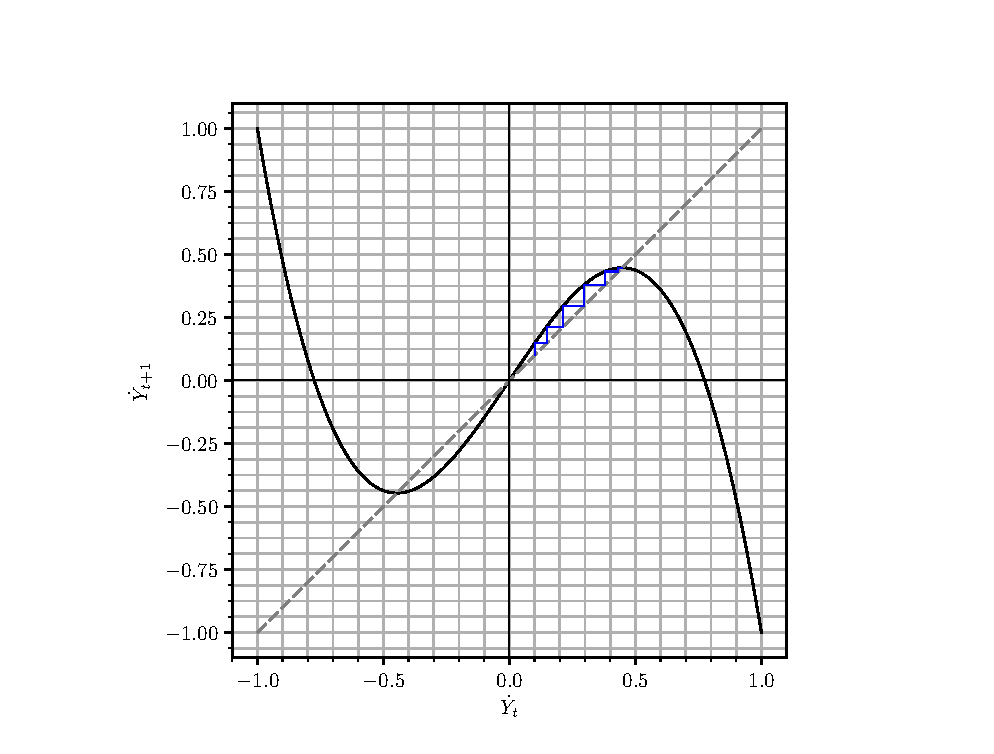
\includegraphics[height=0.4\textheight]{sam_hicks/fixed.eps}
    \caption{Cobweb plot of the multiplier-accelerator model displaying a fixed point at $\dot Y\approx0.447$. $\mu=1.5$ and $\dot Y_0=0.5$}
    \label{mult_fixed}
\end{figure}

When $\mu>2$ the fixed point loses stability; however, the double iterate of the function gains a stable fixed point, i.e. a stable 2-cycle forms. 

\begin{figure}
    \centering
    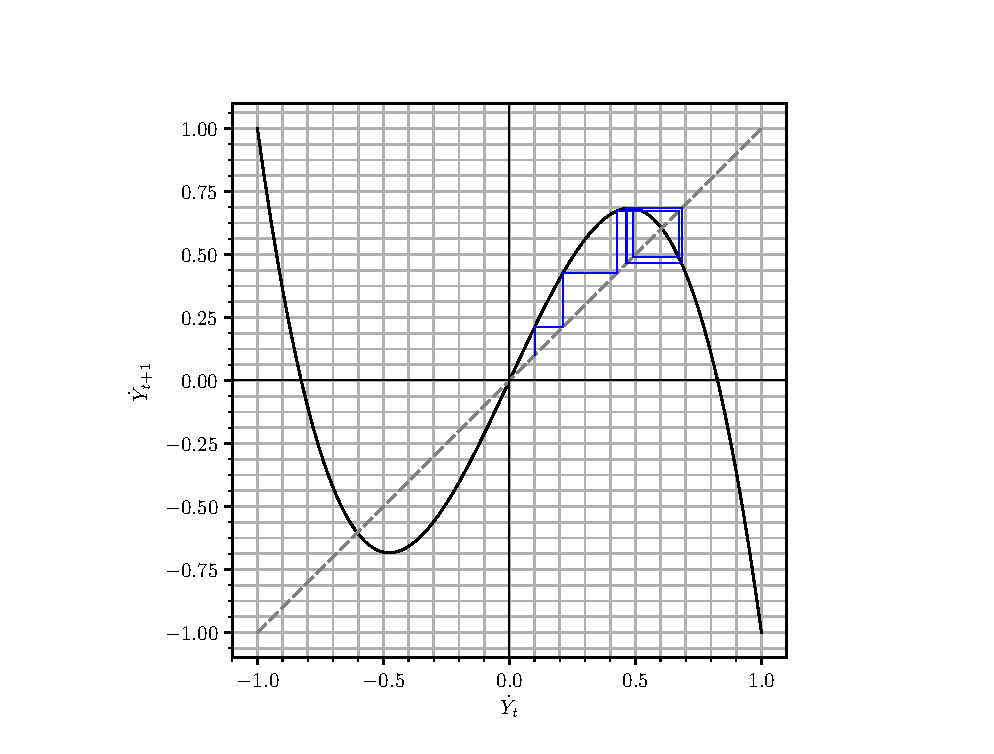
\includegraphics[height=0.4\textheight]{sam_hicks/2-cyclic.eps}
    \caption{Cobweb plot of the multiplier-accelerator model displaying a 2-cycle. $\mu=2.15$ and $\dot Y_0=0.1$}
    \label{mult_2-cycle}
\end{figure}
The parameter range of cycle stability decreases as the periodicity of the cycle increases until $\mu\approx2.302$ which is when this mapping reaches the Feigenbaum constant. Once $\mu$ exceeds this point, the model becomes chaotic; however, it is bound in the quadrant of the original point. The implication of this is that an economy facing growth will continue to encounter growth but an economy that is decaying will always decay.
\begin{figure}
    \centering
    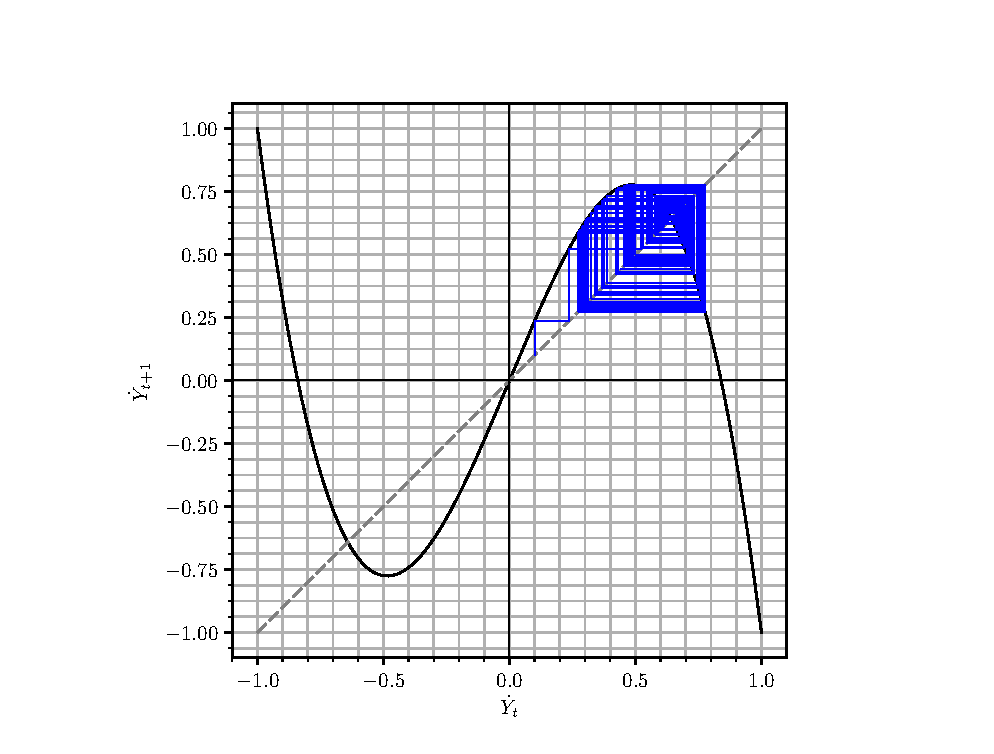
\includegraphics[height=0.4\textheight]{sam_hicks/chaos_contained.eps}
    \caption{Cobweb plot of the multiplier-accelerator model displaying bounded chaos. $\mu=2.4$ and $\dot Y_0=0.1$}
    \label{mult_bounded-chaos}
\end{figure}
It is possible for the mapping to exit the bounds of its quadrant. The value of $\mu$ such that the 0 of the mapping is equal to the maximal point of the mapping marks the transition point between bounded chaotic behavior and "unbounded" chaotic behavior (the mapping is still bounded within [-1, 1]). This occurs when 
\begin{equation*}
    \mu=\frac{3\sqrt{3}}{2}\approx2.5981
\end{equation*}
\begin{figure}
    \centering
    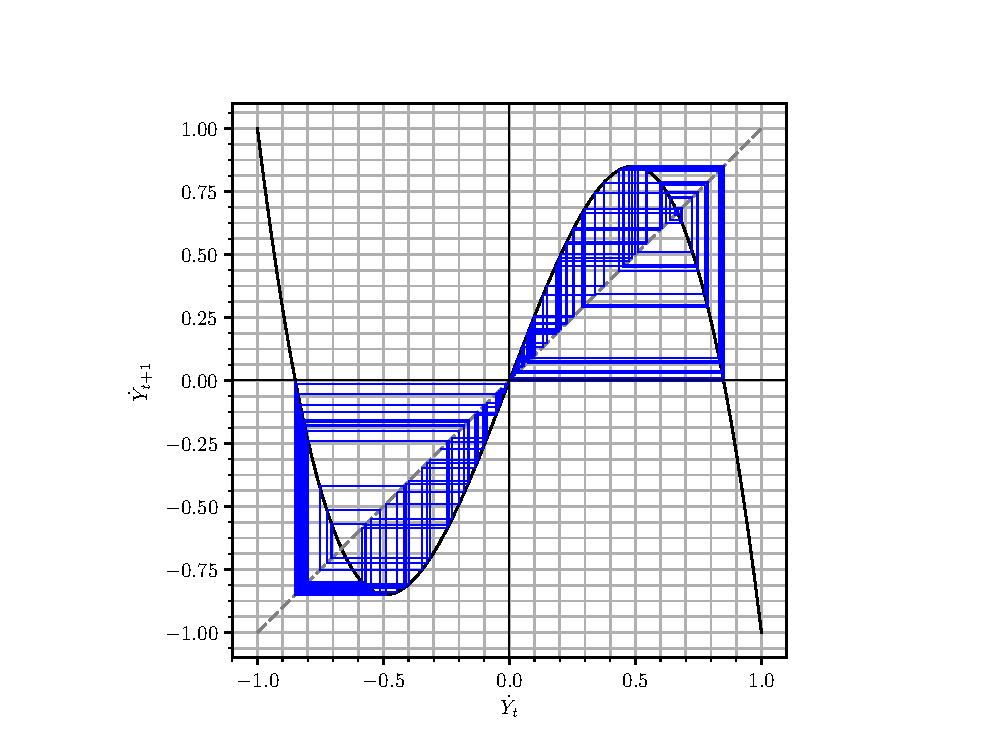
\includegraphics[height=0.4\textheight]{sam_hicks/chaos_uncontained.eps}
    \caption{Cobweb plot of the multiplier-accelerator model displaying bounded chaos. $\mu=2.6$ and $\dot Y_0=0.1$}
    \label{mult_unbounded-chaos}
\end{figure}

\begin{figure}
    \centering
    \includegraphics[height=0.4\textheight]{sam_hicks/bifurcation.eps}
    \caption{Bifurcation diagram of the multiplier-accelerator model varying $\mu$ between 0.9 and 3. The plot constructed using 0.1 as an initial point is displayed in black and the plot constructed using -0.1 as the initial point is displayed in blue. The last 50 points given a 10000 iteration timeseries are displayed.}
    \label{mult_bifurcation}
\end{figure}
Figure \ref{mult_bifurcation} displays the transitions this mapping makes between a stable fixed point, a 2-cycle, 4-cycle and so on until chaotic behavior arises. It is important to note though that even in the chaotic region, there exist windows of order. 
\begin{figure}
    \centering
    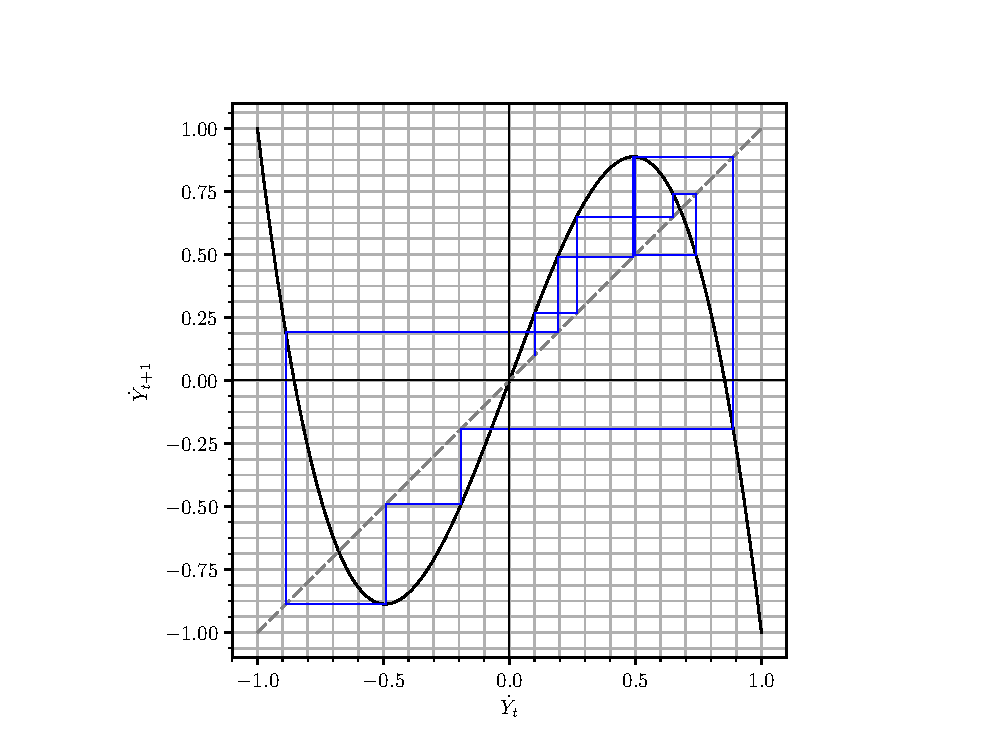
\includegraphics[height=0.4\textheight]{sam_hicks/unbound_cyclic.eps}
    \caption{Cobweb plot of the multiplier-accelerator model displaying a cycle featuring growth and decay. $\mu=2.7$ and $\dot Y_0=0.1$}
    \label{mult_unbound-cycle}
\end{figure}
Figure \ref{mult_unbound-cycle} displays a stable cycle that arises in one such window of order. This cycle is not bounded within its quadrant, it can thus feature endogenous growth and decay in the same cyclic trajectory, which is a significant distinction from all other cycles displayed thus far. 

Although the Feigenbaum point provides sufficient proof of the presence of chaos, it is still useful to plot the Lyapunov exponent in order to determine the exact regions of chaotic behavior.
\begin{figure}
    \centering
    \includegraphics[height=0.4\textheight]{sam_hicks/Lyapunov.eps}
    \caption{Plot of Lyapunov exponent varying $\mu$ using 0.1 as the initial point. $100,000^{th}$ iteration of the mapping is used to computationally solve for the Lyapunov exponent. }
    \label{mult_Lyapunov}
\end{figure}
Figure \ref{mult_Lyapunov} allows us to explicitly identify the parameter ranges of windows of order in the region of chaos. 
\chapter{Conclusion}
One of the core debates of economic theory is that of the rationality of agents. Keynesian economics was the dominant school of thought until the 1970s which saw the rise of New Classical economics\autocite{Hartley2013}. Lucas and Sargent were two key spearheads of this movement with their influential paper titled "After Keynesian Macroeconomics", key to their complaints were the lack of microeconomic foundations in Keynesian models\autocite{Lucas1979}. Real business cycle theory, a major branch of New Classical economics believed that business cycles were a rational response to exogenous shocks to the economy and were perfectly efficient. However, this also meant that business cycles would not arise endogenously as firms and consumers would learn over time the behavior of the economy as they, as a whole, acted rationally. Though Keynesianism has since gained in popularity after the 2007 financial crisis, these lessons of New Classical Economics continue to influence the microfoundations of macroeconomic New Keynesian models.

Wegener, et al. directly based their inventory cycle model on that developed by Metzler. However, both of these models required that firms be boundedly rational which, to a New Classical economist, would be an unrealistic assumption not rooted in microeconomic foundations. However, it is appropriate to limit the ability for firms to predict the future if the reason for it can be appropriately explained. Behavioral economics and experimental data has frequently shown a gap between perfectly rational, utilitarian behavior and what is actually practiced by humans\autocite{Smith2006}; however, we would expect firms to behave more rationally than individuals. Some models make use of stochastic shocks in order to drive dynamic behavior; these tend to follow a New Classical real business cycle framework as these stochastic processes are the primary drivers of economic cycles. Another possible process is that of chaotic behavior. Under these conditions, it is possible for the economy to reside in a completely deterministic state while still making it impossible for firms to accurately predict future states in the economy . Having the unpredictability of the economy be primarily driven by chaotic processes rather than stochastic ones is of great use from a policy perspective due to the nature of having parameters to influence rather than random behavior, this is discussed in greater detail by Faggini and Parziale\autocite{Faggini2012}. 

The growth model described in Chapter \ref{ch:metzlerian-expanded} has a basis in Metzler's inventory cycle but also incorporates a multiplier-accelerator mechanism for endogenous investment and consumption and the results of numerical simulations of the model display the possibility of chaos, in addition to other phenomena such as the existence of multiple attractors. Of particular note is the bifurcation diagram and Lyapunov exponent plot of the parameter $s$. The marginal propensity to save, under the initial conditions and other parameter choice tested, do not display any stable fixed points. In fact, over the possible range of $s$, most possible trajectories are chaotic; one such trajectory is displayed in Figure \ref{growth_chaotic-timeseries}.
\begin{figure}
    \centering
    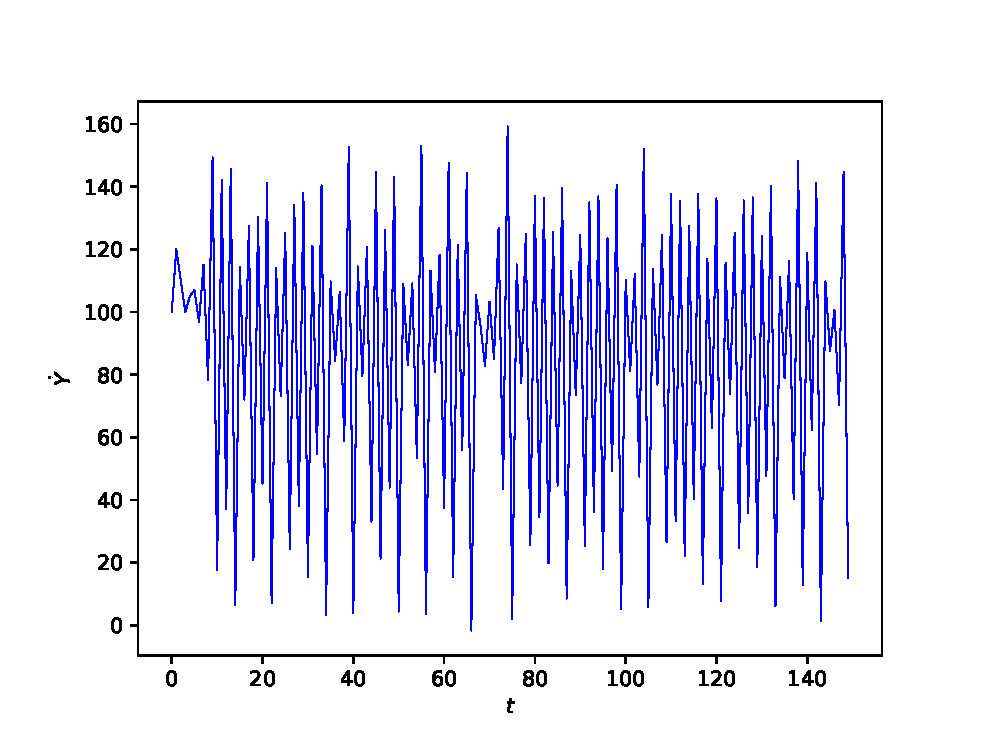
\includegraphics[height=0.4\textheight]{./metzlerian_growth/chaotic_timeseries.eps}
    \caption{Timeseries plot of income growth rate over 150 iterations. $s=0.4,\ k=0.3,\ v=500,\ q=0.001$. Initial values of $\dot Y$ are: 100, 120, 110, 100, 105, 107}
    \label{growth_chaotic-timeseries}
\end{figure}
Figure \ref{metzlerian_growth-kLyapunov} also displays chaotic behavior; however, this only occurs when $k$ is very large and is unlikely to occur in a real scenario. Both $s$ and $k$ are the two parameter choices that describe the behavior of the agents of the economy in non-monetary terms. Based on the results of Figure \ref{metzlerian_growth-kLyapunov} and \ref{metzlerian_growth-kbifurcation}, variation of this parameter has minor effects on the growth rate of the economy compared to variation of $s$. This implies that the choice of inventory proportion, outside of the extreme cases, has a minor impact on the long-run dynamics of the model. This is not to say that the inventory cycle is itself a minor factor of the economy; removal of the inventory cycle changes this model to an unsimplified version of the model presented in Chapter \ref{ch:multiplier-accelerator}. This model features a functionally identical mechanism for consumption with a Robertson lag and although the form of the function for endogenous investment differs between the two models, they are qualitatively similar for the reasons mentioned in Chapter \ref{ch:metzlerian-expanded}.

\begin{figure}
    \centering
    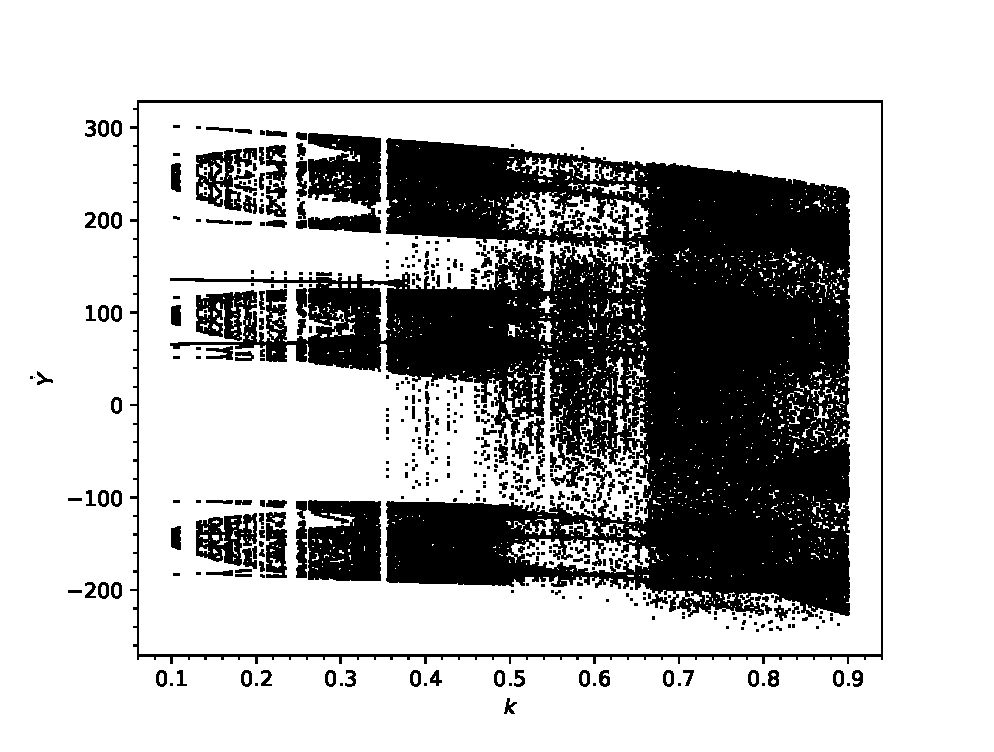
\includegraphics[height=0.4\textheight]{./metzlerian_growth/kbifurcation2.eps}
    \caption{Bifurcation diagram varying $k$ between 0.1 and 0.9. Initial conditions and other parameters are held constant as described in Figure 4.1 except $s=0.7$}
    \label{metzlerian_growth-kbifurcation2}
\end{figure}
\begin{figure}
    \centering
    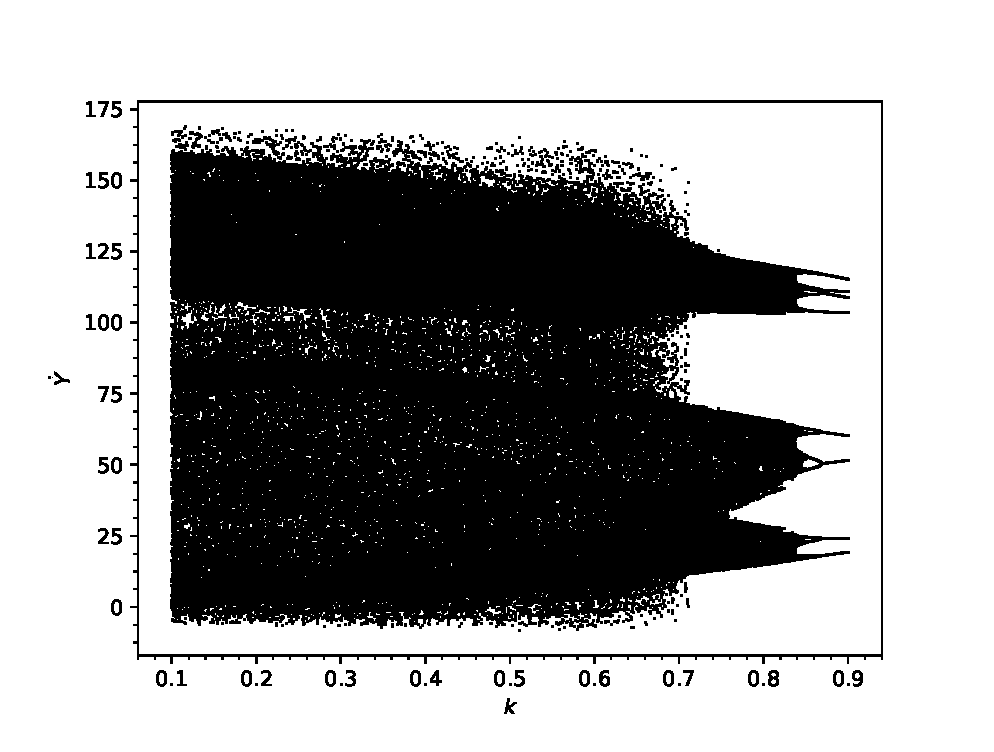
\includegraphics[height=0.4\textheight]{./metzlerian_growth/kbifurcation3.eps}
    \caption{Bifurcation diagram varying $k$ between 0.1 and 0.9. Initial conditions and other parameters are held constant as described in Figure 4.1 except $s=0.3$}
    \label{metzlerian_growth-kbifurcation3}
\end{figure}
Figure \ref{metzlerian_growth-kbifurcation2} and \ref{metzlerian_growth-kbifurcation3} displays behavior that is qualitatively distinct from that in Figure \ref{metzlerian_growth-kbifurcation} despite both plots showing the long-run behavior of the model with the same variation in $k$. However, by increasing or decreasing $s$ until it is in the chaotic regime presented in Figure \ref{metzlerian_growth-sLyapunov}, we see that varying $k$ can have a significant effect on the long-run dynamics of growth at even more reasonable values of $k$.

$q$ determines the maximum and minimum of the investment function and $v$ is the primary determinant of of the FWHM of the function. Given the initial conditions, we see chaotic behavior when large quantities of investment are allowed by the investment curve, i.e. $q$ is small. The initial growth values vary between 100 and 120 so it appears that allowing investment to exceed growth in quantity results in instability;  however, there do still remain windows of order in the primary chaotic region of $q$. Interestingly, the system appears to be relatively ordered for most values of $v$; however, there is a small region where $250<v<750$ that displays chaotic behavior in Figure \ref{metzlerian_growth-vLyapunov}. Figure \ref{metzlerian_growth-chaotic_timeseries2} displays one such trajectory, of note is how the model cycles between both positive and negative growth regimes but also between high amplitude variation and low amplitude variation. It appears that under this parametrization, high absolute values of income change reduce investment; however, instead of ending in stability, this lower income variance state drives higher levels of investment shifting the model back to a high income variance regime.
\begin{figure}
    \centering
    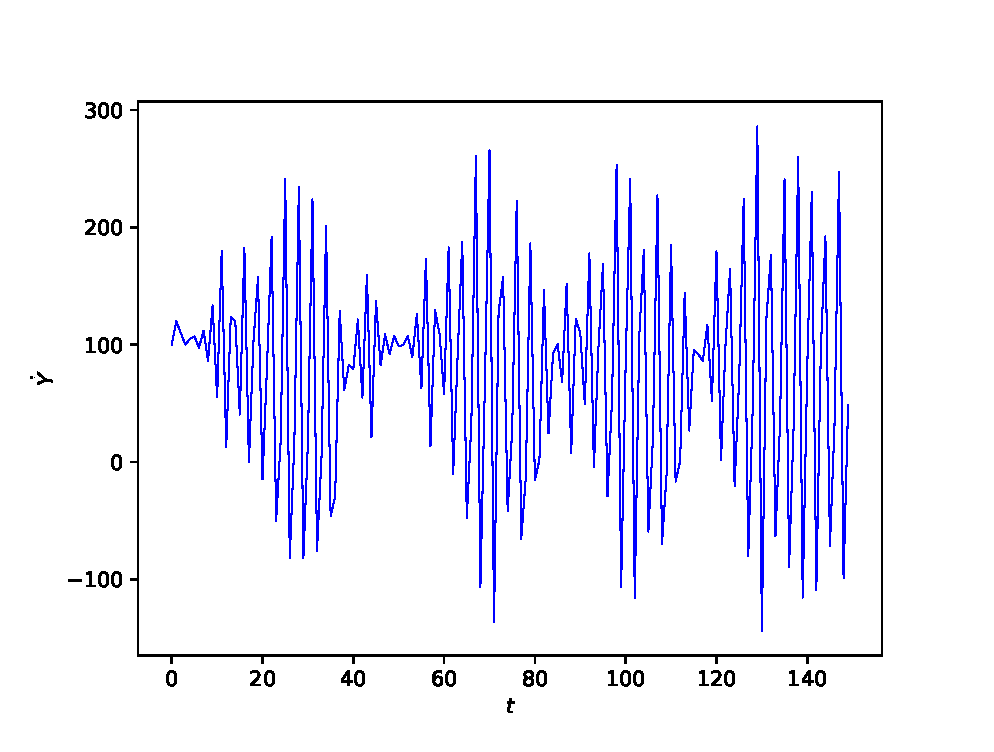
\includegraphics[height=0.4\textheight]{./metzlerian_growth/chaotic_timeseries2.eps}
    \caption{Timeseries plot of income growth rate over 150 iterations. $s=0.6,\ k=0.3,\ v=416,\ q=0.001$}
    \label{metzlerian_growth-chaotic_timeseries2}
\end{figure}

$v$ and $q$ are likely to change depending on the state of the economy, the government's fiscal policy, and the technology available. The investment curve bends back and has a "width" due to the presumption of changes in public investment and taxes in response to the state of the economy and the presence of other limiting factors in income growth. If the government decides to loosen their concern to output variation, the width of the investment curve would increase. The height of the function can change over time as the required level of investment needed to sustain an output level changes can change with improvements in technology or human capital. 

Generally speaking, larger values of early initial growth compared to the later values of initial growth results in a lower overall long-run growth. This can be seen in Figure \ref{metzlerian_growth-y0bifurcation}, \ref{metzlerian_growth-y1bifurcation}, and \ref{metzlerian_growth-y2bifurcation}. The relationship is reversed if growth is larger for more recent time periods as can be seen in Figure \ref{metzlerian_growth-y3bifurcation}, \ref{metzlerian_growth-y4bifurcation}, and \ref{metzlerian_growth-y5bifurcation}. Ignoring the chaotic behavior, this model implies that relatively sharp drops in growth rate result in lower growth horizons whereas large spikes in growth rate result in high growth horizons. The non-linear nature of the model and presence of multiple attractors complicates this idea although the trend is still present. This economy is susceptible to external forces; an exogenous but temporary increase in the growth rate will result in a long-run increase in growth rate. The economy is thus able to use aid in order to accelerate its own growth. Likewise, if an external shock reduces output relative to its usual behavior, this can result in a decreased growth rate in the long-run. 

The goal of this model was to incorporate both a Robertson and Lundberg lag and endogenize investment change. This was done in order to provide a mechanism to explain why firms on aggregate are unable to accurately predict future consumption. Many models use stochastic processes in order to rationalize this; however, this model shows the presence of chaotic behavior. Under a chaotic regime, firms would only be able to predict future behavior by knowing the exact state of the economy in the past; however, this is practically impossible as even small differences between the actual initial conditions and estimated initial conditions will result in very different future results by the definition of chaos. 

Much work remains to be done on this model in order to better describe the quantity and structure of the multiple attractors and an explanation of the model's response to changing parameters. As more work is done on the mathematics of higher-order non-linear iterated maps, it may become possible to analytically solve for the behavior of the model although this remains unlikely for the near future. More work also needs to be done to differentiate between quasi-periodic behavior and chaotic behavior in the model, although both are inherently unpredictable, quasi-periodic behavior provides a more consistent structure to long-run behavior while still preventing firms from accurately determining future outcomes.

This model could also be expanded upon in a variety of ways. This economy is closed; however, most modern economies are open to foreign trade to varying degrees. This provides another income channel as well as providing another outlet for investment that does not improve the domestic economy. A more complex investment mechanism could also be incorporated, by explicitly separating public and private investments and removing the x-axis symmetry seen in the current curve. There are many possible ways for firms to predict future consumption, a simple average was used here although a conditional expectation that would allow firms to better use past information and learn from their previous experiences would help alleviate concerns regarding rational behavior by the firms. This however can lead to mathematical complications if firms have infinite possible memory. These additions could improve the realism of the model while still using chaos as the primary driver of chaotic behavior. 




\chapter{References}
\thispagestyle{empty}
\printbibliography[heading=none]

\end{document}
